\section{Main Screen}
\begin{figure}[H]
    \centering
    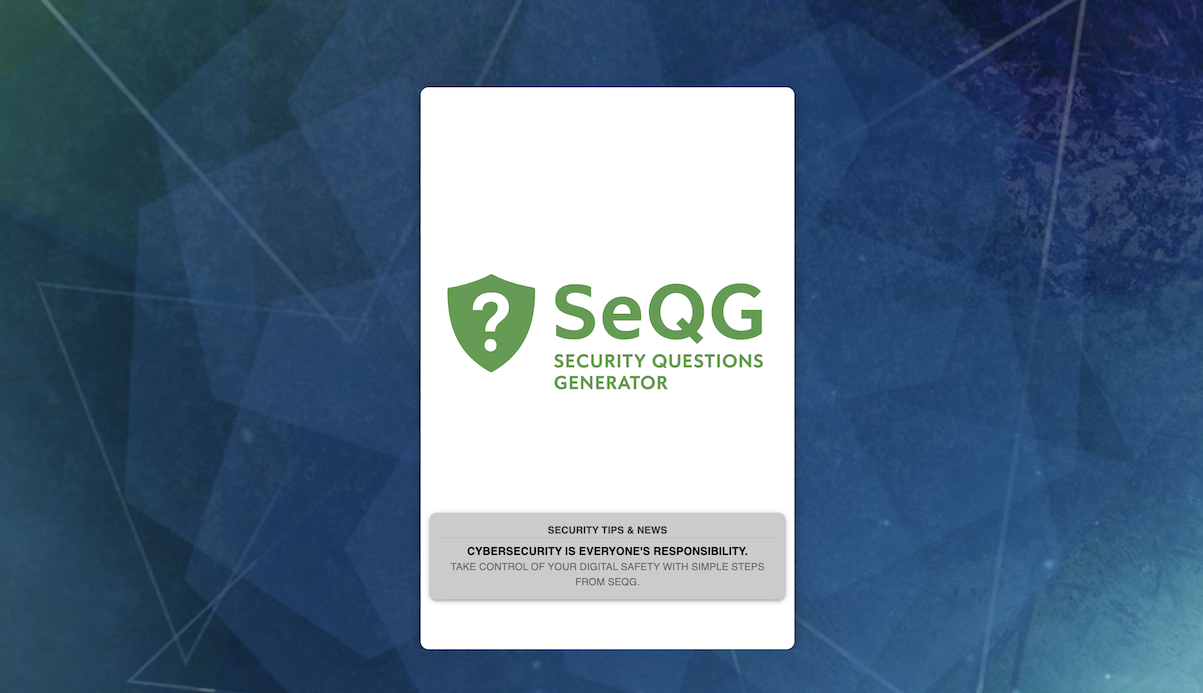
\includegraphics[width=0.8\textwidth]{images/MainScreen1.png}
    \caption{Main Screen}
\end{figure}

When the system is offline, the display shows a static screen where \textbf{security tips and news} are 
dynamically fetched by the LLM. These messages, shown in Figure 2.1, are designed to catch users’ attention 
and encourage them to engage with \textbf{SeQG} and learn more about \textbf{cybersecurity}.

\begin{figure}[H]
    \centering
    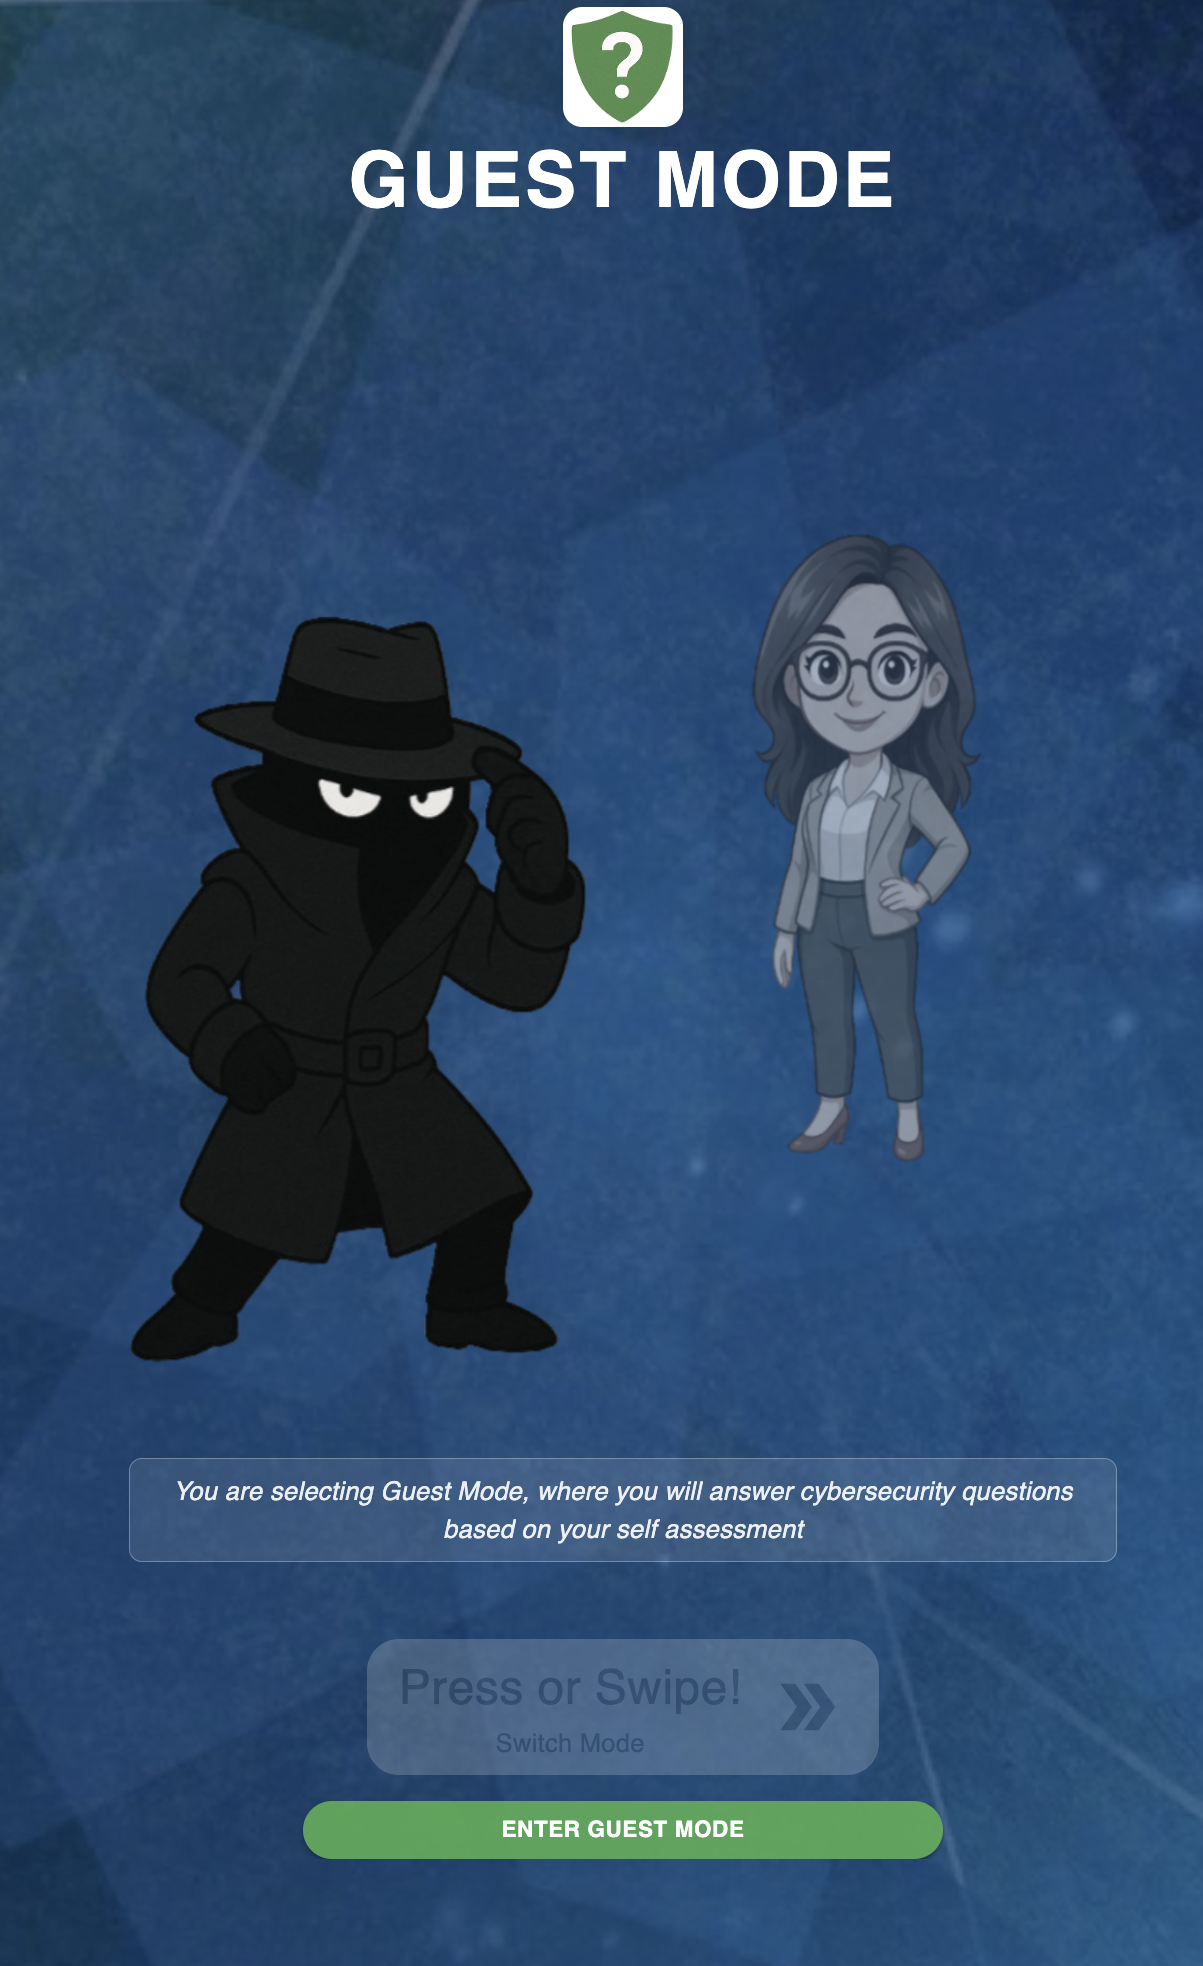
\includegraphics[width=0.4\textwidth]{images/MainScreenCharacter1.png}
    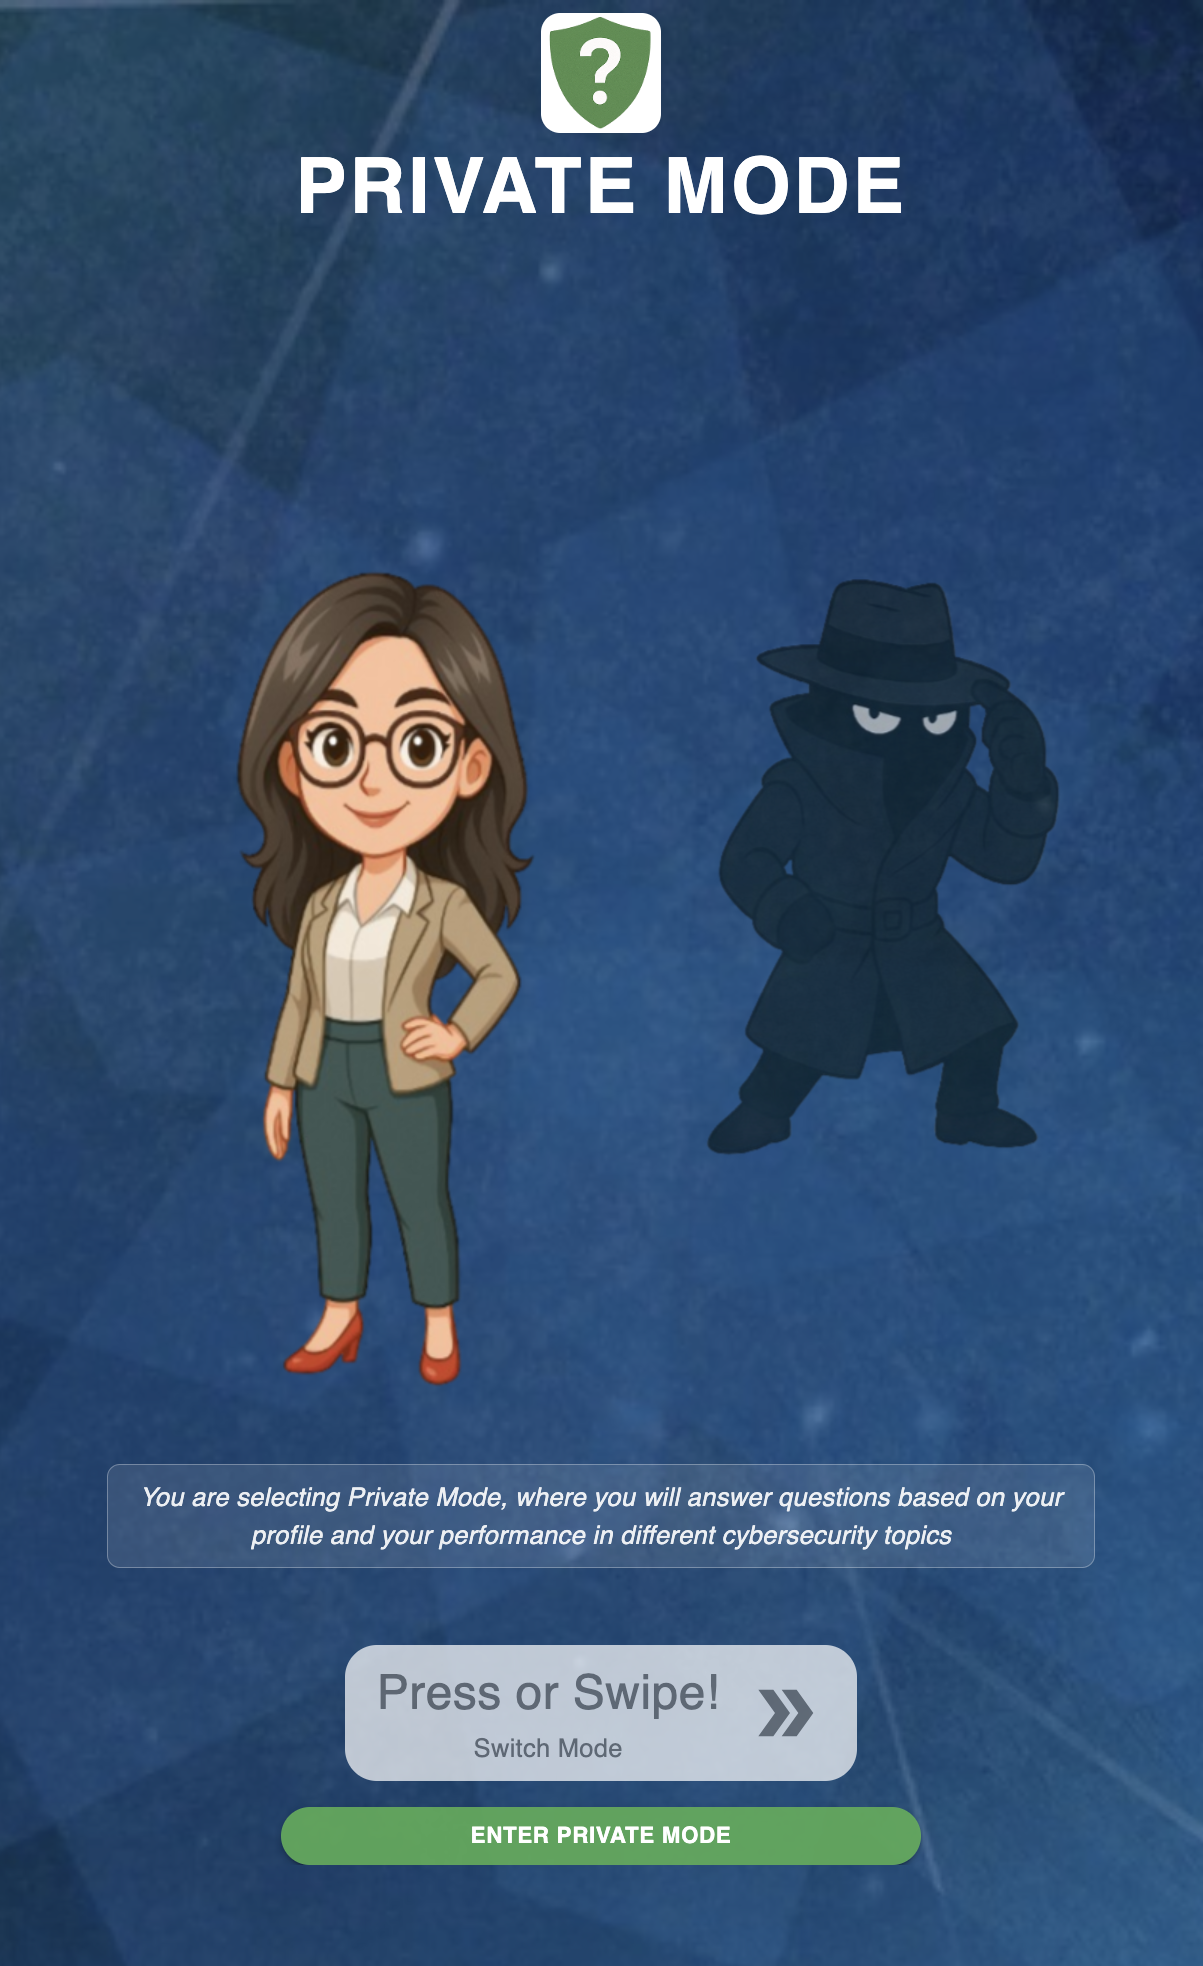
\includegraphics[width=0.4\textwidth]{images/MainScreenCharacter2.png}
    \caption{Characters for Mode selection}
\end{figure}
When a user approaches the display and taps the screen, \textbf{two mode characters} appear, each accompanied 
by a short explanation of their functionality, as to be seen in Figure 2.3.